%----------------------ELEMENTOS PÓS-TEXTUAIS----------------------%
\postextual

%--------------------Referências Bibliográficas--------------------%
\bibliography{bibliografia}


%-----------------------------Apêndices-----------------------------%
\begin{apendicesenv}

\chapter{Tutorial Básico de \LaTeX}

\section*{Introdução}
\LaTeX{} é um sistema de preparação de documentos de alta qualidade tipográfica, amplamente utilizado em publicações científicas e acadêmicas. Este tutorial oferece uma introdução detalhada ao \LaTeX, cobrindo os conceitos e comandos fundamentais para a criação de documentos profissionais.

\section*{Estrutura Básica de um Documento}
Um documento \LaTeX{} típico possui a seguinte estrutura básica:

\begin{verbatim}
\documentclass{classe}
\usepackage{pacotes}

\begin{document}
    % Conteúdo do documento
\end{document}
\end{verbatim}

\begin{itemize}
    \item \texttt{\textbackslash documentclass\{classe\}}: Define a classe do documento (e.g., \texttt{article}, \texttt{report}, \texttt{book}).
    \item \texttt{\textbackslash usepackage\{pacotes\}}: Inclui pacotes adicionais para funcionalidades extras.
    \item \texttt{\textbackslash begin\{document\}} e \texttt{\textbackslash end\{document\}}: Delimitam o início e o fim do conteúdo do documento.
\end{itemize}

\section*{Texto e Formatação}
Você pode escrever texto normalmente e utilizar comandos para formatação. Alguns exemplos:

\subsection*{Negrito e Itálico}
\begin{itemize}
    \item \texttt{\textbackslash textbf\{texto em negrito\}}: \textbf{texto em negrito}
    \item \texttt{\textbackslash textit\{texto em itálico\}}: \textit{texto em itálico}
\end{itemize}

\subsection*{Listas}
\LaTeX{} permite criar listas numeradas e não numeradas:

\subsubsection*{Lista Não Numerada}
\begin{verbatim}
\begin{itemize}
    \item Item 1
    \item Item 2
\end{itemize}
\end{verbatim}

\begin{itemize}
    \item Item 1
    \item Item 2
\end{itemize}

\subsubsection*{Lista Numerada}
\begin{verbatim}
\begin{enumerate}
    \item Primeiro item
    \item Segundo item
\end{enumerate}
\end{verbatim}

\begin{enumerate}
    \item Primeiro item
    \item Segundo item
\end{enumerate}

\section*{Equações Matemáticas}
Uma das grandes vantagens do \LaTeX{} é a facilidade para escrever equações matemáticas. Uma lista de símbolos matemáticos geralmente utilizados desenvolvida por \citeonline{heinken20XXlatex} pode ser encontrada no Anexo \ref{anexo:symbols}.

\subsection*{Equação em Linha}
Use o símbolo \texttt{\$} para delimitar equações em linha. Por exemplo, para obter o seguinte resultado \( E = mc^2 \), escreva \verb|$ E = mc^2 $|.

\subsection*{Equação em Bloco}
Para equações em bloco, use o ambiente \texttt{equation}:

\begin{verbatim}
\begin{equation}
    E = mc^2
\end{equation}
\end{verbatim}

\begin{equation}
    E = mc^2
\end{equation}

\subsection*{Equações Multilinhas}
Para equações que se estendem por várias linhas, use o ambiente \texttt{align} do pacote \texttt{amsmath}:

\begin{verbatim}
\begin{align}
    a &= b + c \\
    d &= e + f
\end{align}
\end{verbatim}

\begin{align}
    a &= b + c \\
    d &= e + f
\end{align}

\section*{Inserção de Imagens}
Você pode inserir imagens com o pacote \texttt{graphicx}:

\begin{verbatim}
\begin{figure}[H]
    \centering
    \caption{Legenda da imagem}
    \includegraphics[width=0.5\textwidth]{example-image}
    \\
    \caption*{\small{Fonte: Autor (20XX)}}
    \label{fig:exemplo}
\end{figure}
\end{verbatim}

\begin{figure}[H]
    \centering
    \caption{Legenda da imagem}
    \includegraphics[width=0.5\textwidth]{example-image}
    \\
    \caption*{\small{Fonte: Autor (20XX)}}
    \label{fig:exemplo}
\end{figure}

\section*{Inserção de Tabelas}

A tabela é uma forma  de apresentação de informações, na qual o dado numérico é o principal elemento de destaque. Caracteriza-se por apresentar dados dispostos em linhas e colunas, organizados em uma estrutura que facilita a visualização e a comparação das informações \cite{ManualIBGE}. 

O código abaixo exemplifica como incluir uma tabela em \LaTeX. O resultado é mostrado logo em seguida:

\begin{verbatim}
\begin{table}[H]
    \centering
    \caption{Exemplo de Tabela de Dados Numéricos}
    \begin{tabular}{c c c}
        \hline
        \textbf{Ano} & \textbf{Valor 1} & \textbf{Valor 2} \\
        \hline
        2020 & 1234 & 5678 \\
        2021 & 2345 & 6789 \\
        2022 & 3456 & 7890 \\
        2023 & 4567 & 8901 \\
        \hline
    \end{tabular}
    \\
    \caption*{\small{Fonte: Autor (20XX)}}
    \label{tab:exemplo}
\end{table}
\end{verbatim}

\begin{table}[H]
    \centering
    \caption{Exemplo de Tabela de Dados Numéricos}
    \begin{tabular}{c c c}
        \hline
        \textbf{Ano} & \textbf{Valor 1} & \textbf{Valor 2} \\
        \hline
        2020 & 1234 & 5678 \\
        2021 & 2345 & 6789 \\
        2022 & 3456 & 7890 \\
        2023 & 4567 & 8901 \\
        \hline
    \end{tabular}
    \\
    \caption*{\small{Fonte: Autor (20XX)}}
    \label{tab:exemplo}
\end{table}

\section*{Referências Cruzadas}

Você pode criar referências cruzadas para seções, figuras, tabelas, equações, etc. usando \texttt{\textbackslash label} e \texttt{\textbackslash ref}. No exemplo de inserção de figuras acima, esta foi utilizado o comando \verb|\label{fig:exemplo}|, em que \verb|fig:exemplo| é um ``identificador'' (que deve ser único) da imagem. Assim, para referenciá-la, escreva: \verb|Conforme Figura \ref{fig:exemplo}| para obter o resultado: ``Conforme Figura \ref{fig:exemplo}''.


\chapter{Tutorial de uso do modelo de dissertação Profmat/UFT}

Este Modelo de Dissertação foi construído em \LaTeX , utilizando a classe \abnTeX. Foram realizadas customizações que tornam modelo compatível com as Normas da Associação Brasileira de Normas Técnicas (ABNT), com o Manual de Normas de Apresentação Tabular do Instituto Brasileiro de Geografia e Estatística \cite{ManualIBGE}, além de estar em concordância com o Manual de normalização para elaboração de trabalhos acadêmico-científicos da Universidade Federal do Tocantins \cite{ManualUFT}. Foram realizadas customizações para adequá-lo às versões mais recentes das normas de padronização citadas.

\section*{Apresentação do modelo de dissertação}

Neste tutorial, será apresentada a estrutura básica do modelo a fim de facilitar sua utilização. O modelo está disponível como um \textit{Template} na plataforma Overleaf no seguinte endereço eletrônico: LINK. A abrir o link em sua conta Overleaf, o usuário terá acesso a uma tela semelhante à mostrada na  Figura \ref{fig:estrutura}.

\begin{figure}[H]
    \centering
    \caption{Modelo de Dissertação aberto no editor online Overleaf}
    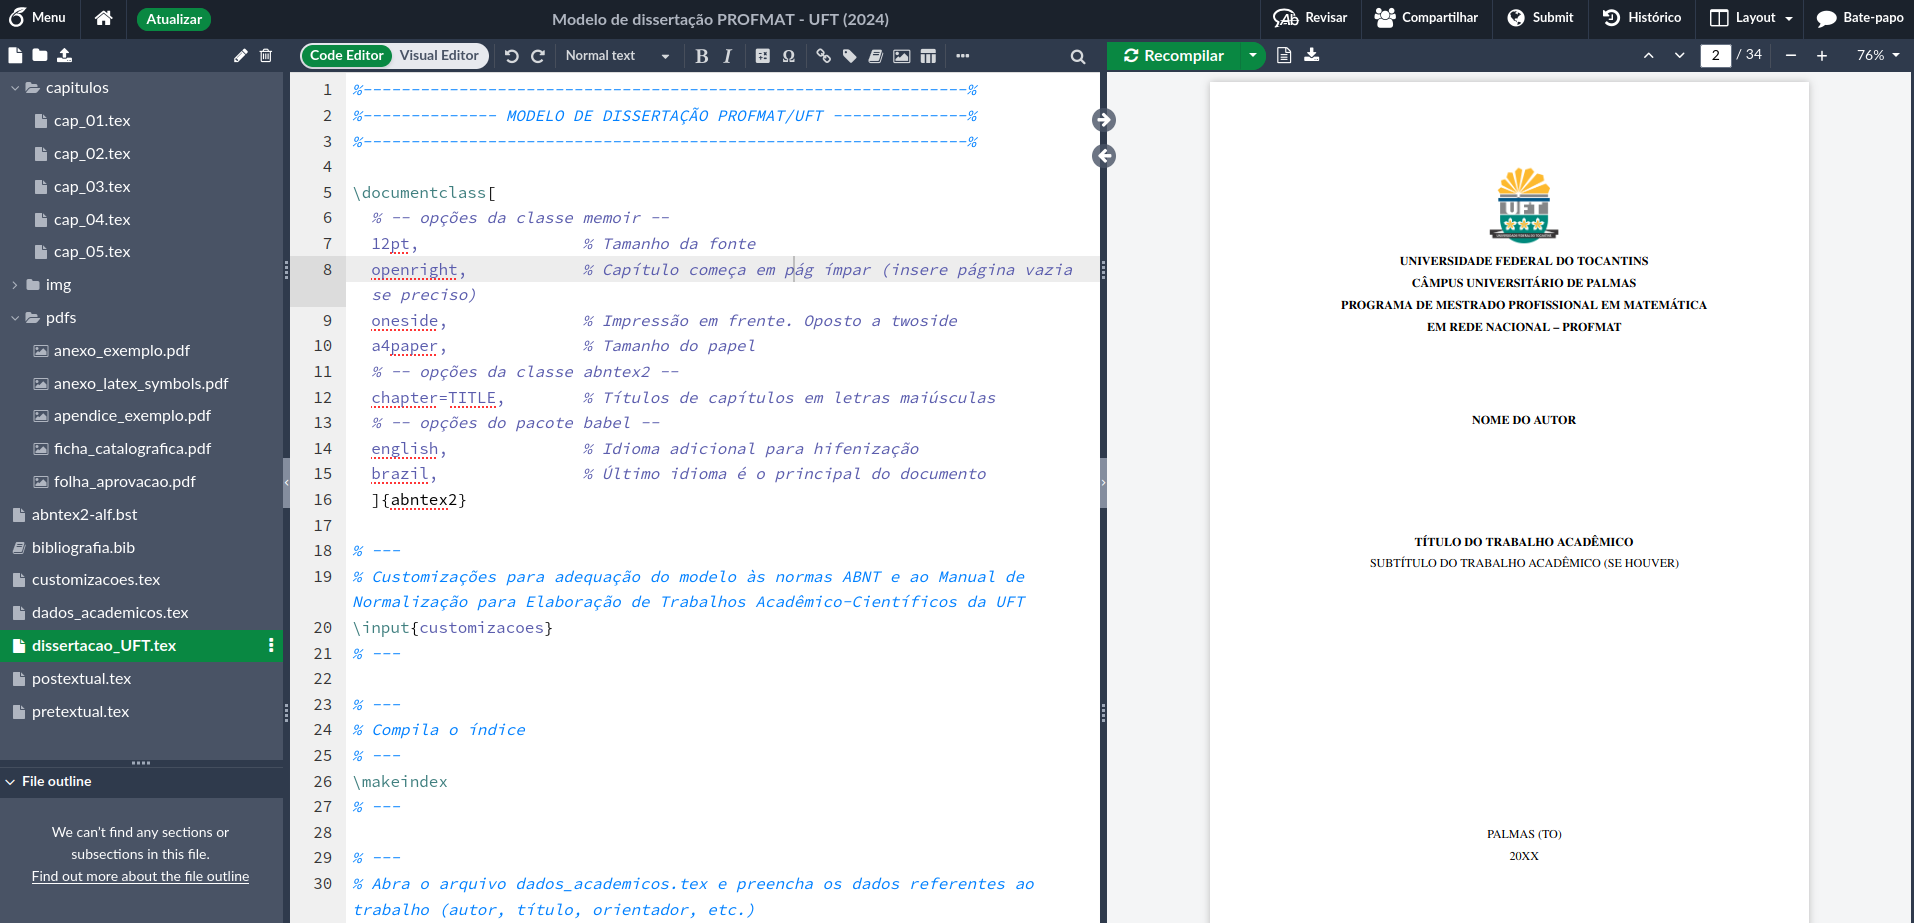
\includegraphics[width=0.9\textwidth]{img/modelo/estrutura_arquivos.png}
    \\
    \caption*{\small{Fonte: Autor (20XX)}}
    \label{fig:estrutura}
\end{figure}

A imagem mostra uma interface de um editor de LaTeX online  Overleaf. O editor está dividido em três seções:  Na coluna da esquerda encontra-se a estrutura de arquivos de um projeto de dissertação, com destaque para o arquivo principal: \verb|dissertação_UFT.tex|. A coluna central mostra o documento atualmente aberto (nesse caso, o código-fonte do arquivo principal). Por fim, a coluna direita apresenta uma visualização prévia do arquivo PDF produzido. 

A estrutura de arquivos da coluna esquerda é resumida a seguir:
    \begin{itemize}
        \item \verb|capitulos/|: Pasta contendo os arquivos dos capítulos da dissertação (\verb|cap_01.tex|, \verb|cap_02.tex|, etc.).
        \item \verb|img/|: Pasta para armazenar imagens, embora esteja colapsada e não possamos ver o conteúdo.
        \item \verb|pdfs/|: Pasta contendo vários PDFs, como anexos e apêndices (\verb|anexo_exemplo.pdf|, \verb|anexo_latex_symbols.pdf|, etc.).
        \item \verb|abntex2-alf.bst|: Arquivo de estilo de bibliografia.
        \item \verb|bibliografia.bib|: Arquivo BibTeX contendo referências bibliográficas.
        \item \verb|customizacoes.tex|: Arquivo contendo customizações específicas para o projeto.
        \item \verb|dados_academicos.tex|: Arquivo contendo informações acadêmicas (autor, título, orientador, etc.).
        \item \verb|dissertacao_UFT.tex|: Arquivo principal do documento LaTeX. É aconselhado que esteja com esse arquivo aberto sempre que necessitar \textbf{Recompilar} seu projeto.
        \item \verb|postextual.tex| e \verb|pretextual.tex|: Arquivos para as partes pré-textuais e pós-textuais do documento.
    \end{itemize}

Nas seções seguintes, apresentamos uma sugestão de sequência de preenchimento do modelo para o desenvolvimento de sua dissertação.

\section*{Dados Acadêmicos}

Abra o arquivo \verb|dados_academicos.tex| e preencha as os campos referentes ao título da dissertação, subtítulo (caso não haja subtítulo, basta a pagar a linha correspondente a esse campo), autor, orientador, instituição, câmpus e data. Os campos referentes ao tipo de trabalho e preâmbulo podem ser deixados como estão pois tratam-se de texto padrão. A Figura \ref{fig:dados-academicos} ilustra um exemplo de preenchimento com dados fictícios.

\begin{figure}[H]
    \centering
    \caption{Preenchimento dos dados acadêmicos}
    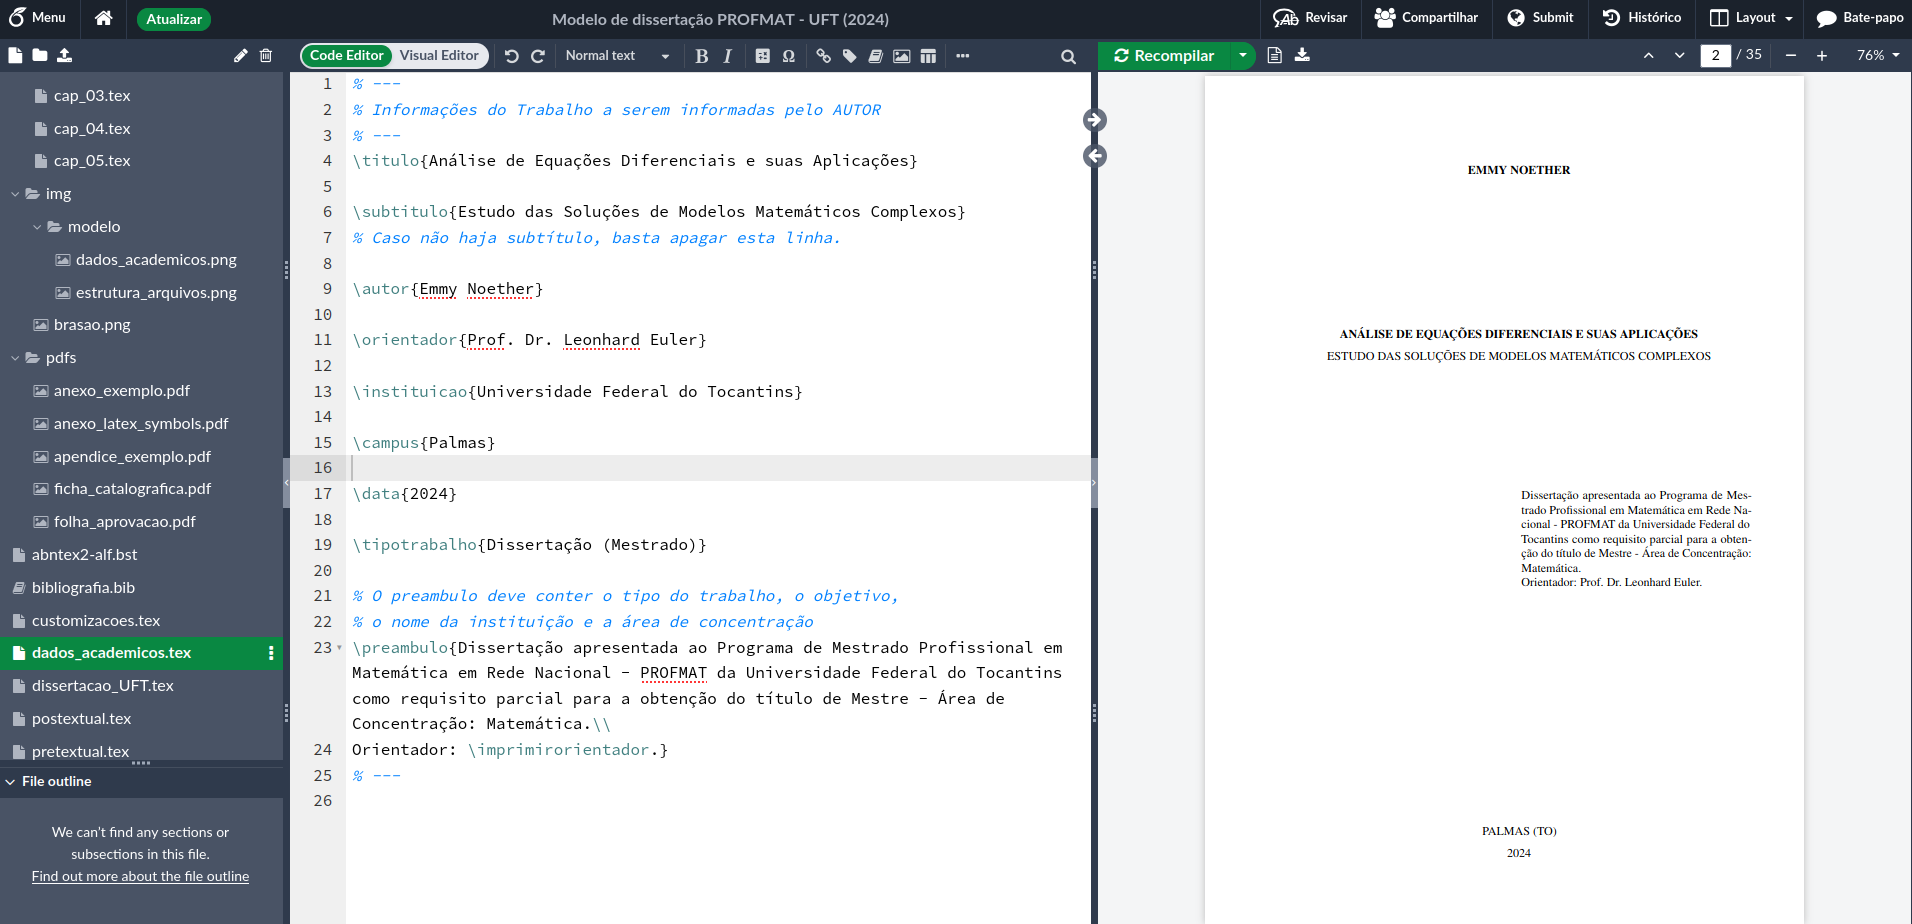
\includegraphics[width=0.9\textwidth]{img/modelo/dados_academicos.png}
    \\
    \caption*{\small{Fonte: Autor (20XX)}}
    \label{fig:dados-academicos}
\end{figure}

Ao clicar no botão \textbf{Recompilar} do editor, os dados informados serão automaticamente carregados nos campos correspondentes tanto da capa quanto na folha de rosto do trabalho.

\section*{Elementos pré-textuais}

Os elementos pré-textuais são as partes iniciais de um trabalho acadêmico que antecedem o conteúdo principal. Eles são fundamentais para a estrutura e apresentação do documento, fornecendo informações essenciais sobre o trabalho, seus autores e orientadores, bem como a instituição\footnote{Para mais detalhes sobre os elementos pré-textuais (obrigatórios e opcionais), leia a norma ABNT NBR 14724 \cite{nbr14724}}.

Abra o arquivo \verb|pretextual.tex|. A seguir, mostra-se o preenchimento das principais informações pré-textuais.

A Figura \ref{fig:pretextual-01} mostra os primeiros quatro elementos pré-textuais: Capa, Folha de rosta, Ficha catalográfica e Folha de aprovação. Quanto aos dois primeiros, nenhuma intervenção é necessário pois são elementos de formatação padronizada cujos dados foram informados no arquivo \verb|dados_academicos.tex| como detalhado na seção anterior.

\begin{figure}[H]
    \centering
    \caption{Elementos pré-textuais: Ficha catalográfica e Folha de aprovação}
    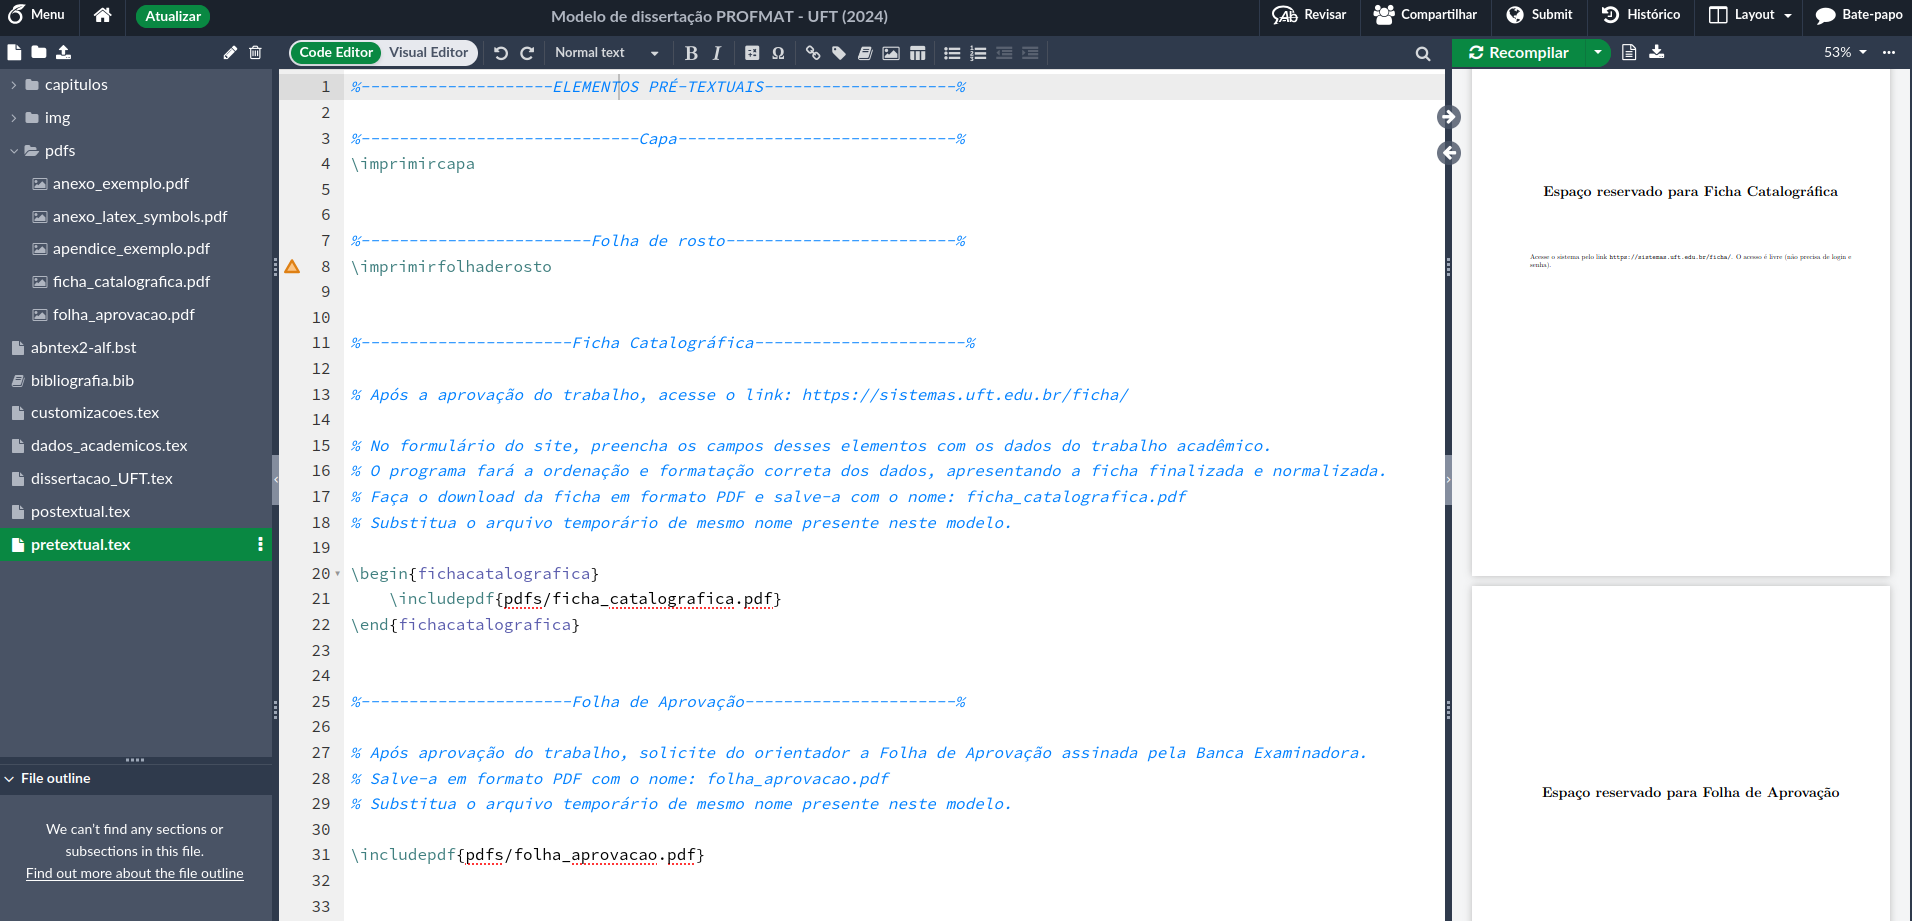
\includegraphics[width=0.9\textwidth]{img/modelo/pretextual-01.png}
    \\
    \caption*{\small{Fonte: Autor (20XX)}}
    \label{fig:pretextual-01}
\end{figure}

A respeito da Ficha Catalográfica e da Folha de Aprovação, tratam-se de documentos cujo preenchimento ocorrerá após a aprovação do trabalho e as correções sugeridas pela Banca Examinadora. Após isso, siga o procedimento descrito a seguir:

\subsection*{Ficha Catalográfica}
Após a aprovação do trabalho, acesse o link: \url{https://sistemas.uft.edu.br/ficha/}. No formulário do site, preencha os campos desses elementos com os dados do trabalho acadêmico.  O programa fará a ordenação e formatação correta dos dados, apresentando a ficha finalizada e normalizada. Faça o download da ficha em formato PDF e salve-a com o nome: \verb|ficha_catalografica.pdf| dentro da pasta \verb|pdfs|. 

\subsection*{Folha de Aprovação}

Após aprovação do trabalho, solicite do orientador a Folha de Aprovação assinada pela Banca Examinadora. Salve-a em formato PDF com o nome: \verb|folha_aprovacao.pdf|. Substitua o arquivo temporário de mesmo nome presente na pasta \verb|pdfs| neste modelo.


Nos dois casos acima, esteja atento para o correto nome de arquivos, bem como o local em que devem ser salvos. Ao clicar em \textbf{Recompilar}, os novos arquivos serão carregados em seu trabalho.

Os próximos elementos pré-textuais são: Dedicatória, Agradecimentos e Epígrafe. Seu preenchimento é bastante intuitivo, conforme mostrado na Figura \ref{fig:pretextual-02}.

\begin{figure}[H]
    \centering
    \caption{Elementos pré-textuais: Dedicatória, Agradecimentos e Epígrafe}
    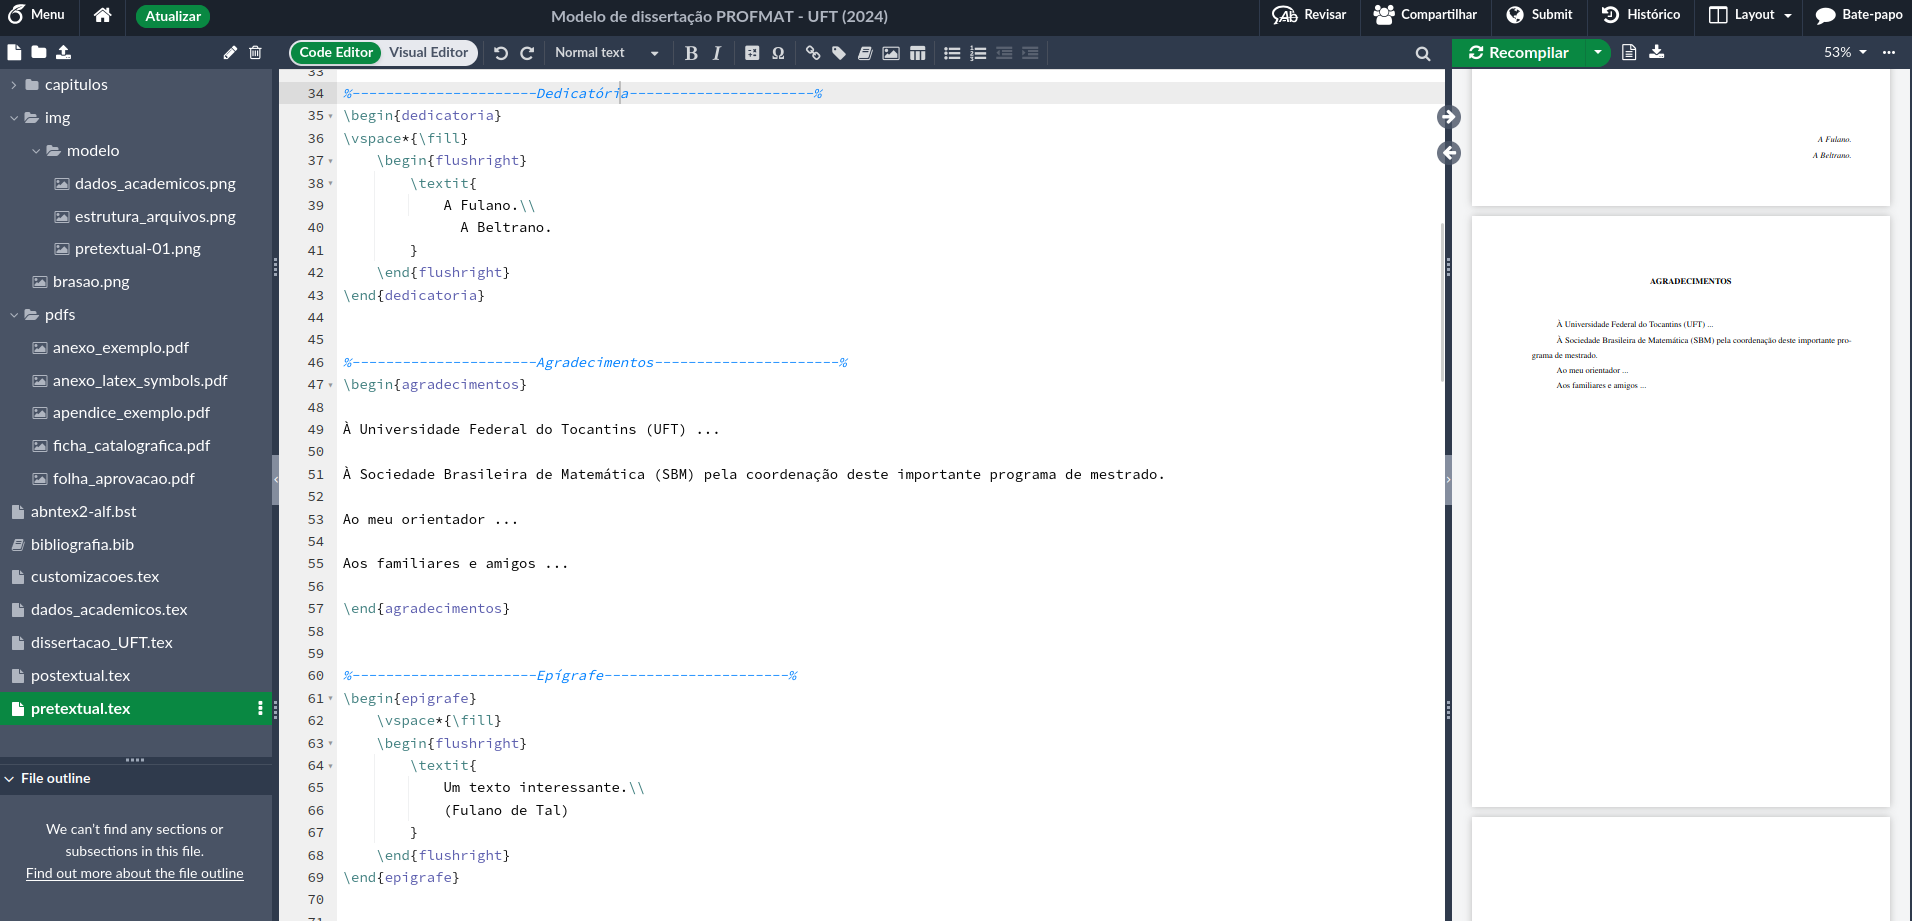
\includegraphics[width=0.9\textwidth]{img/modelo/pretextual-02.png}
    \\
    \caption*{\small{Fonte: Autor (20XX)}}
    \label{fig:pretextual-02}
\end{figure}


Em seguida, tem-se o resumo (em língua portuguesa e em língua estrangeira), conforme mostrado na Figura \ref{fig:pretextual-03}. Observe que de acordo com a norma ABNT NBR 6028:2021 o resumo deve apresentar o conteúdo do trabalho de  forma sucinta, composto por uma sequência de frases concisas em parágrafo único, sem enumeração de tópicos e escritas com verbo na terceira pessoa \cite{nbr6028}.

\begin{figure}[H]
    \centering
    \caption{Elementos pré-textuais: Resumo}
    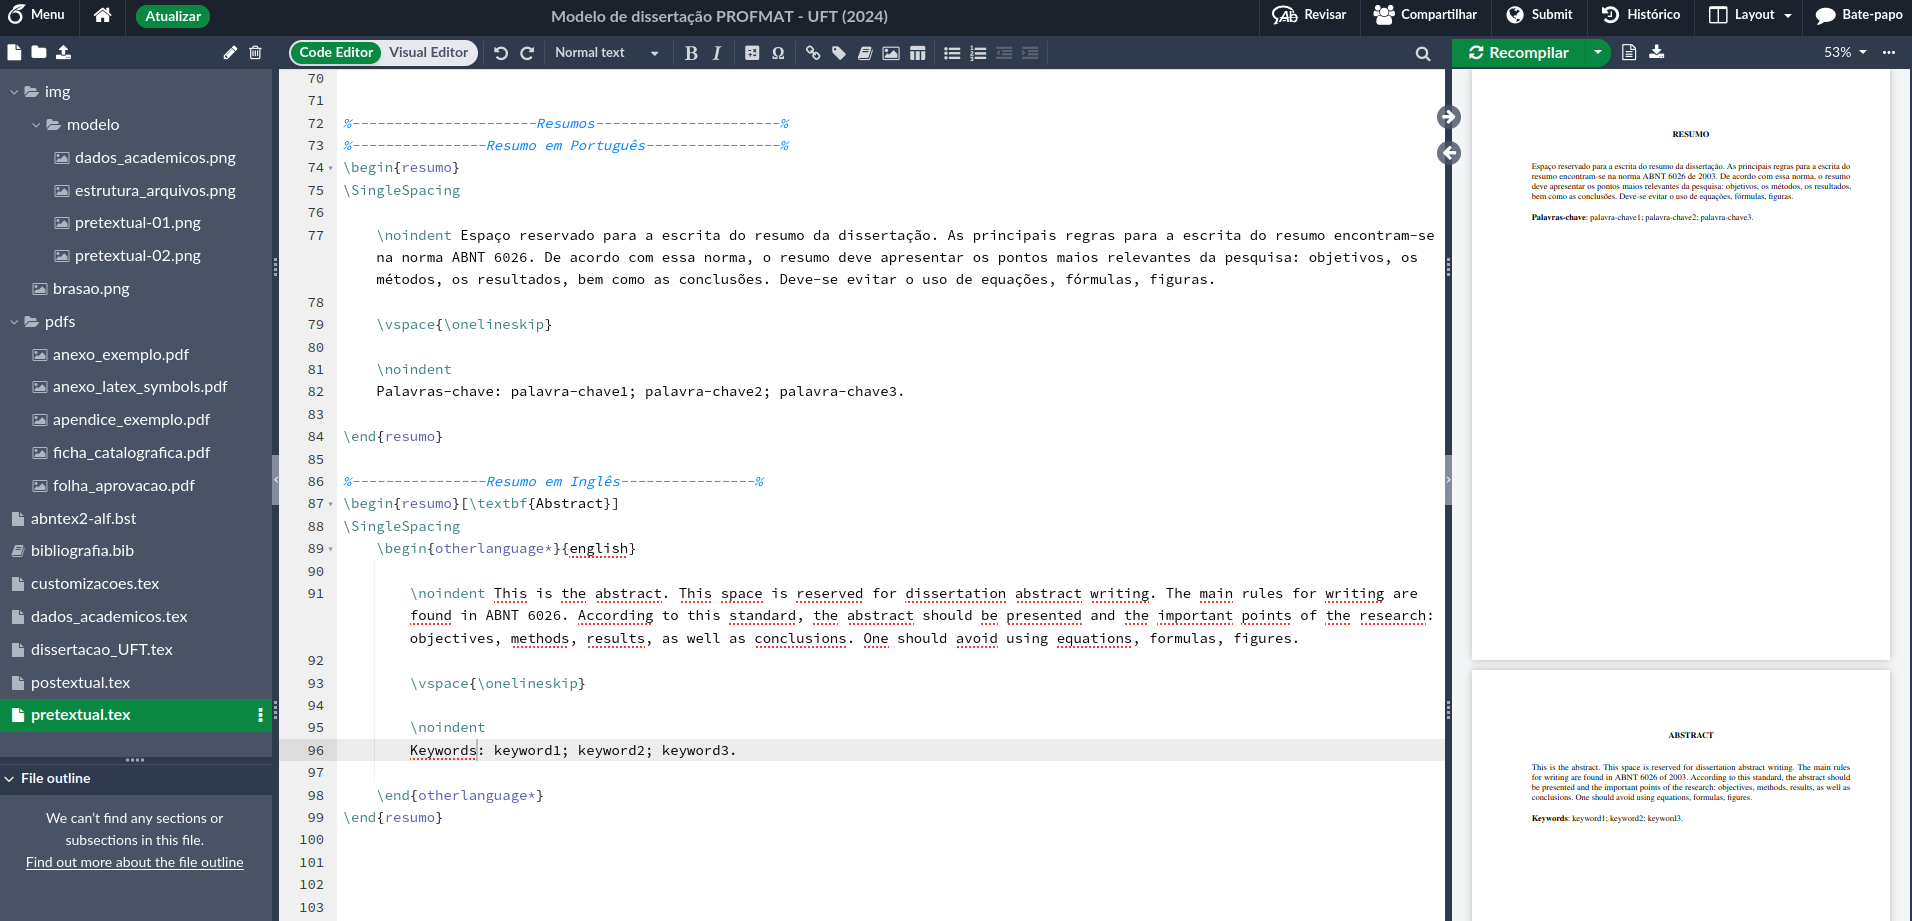
\includegraphics[width=0.9\textwidth]{img/modelo/pretextual-03.png}
    \\
    \caption*{\small{Fonte: Autor (20XX)}}
    \label{fig:pretextual-03}
\end{figure}

Quanto às palavras-chave, segundo a norma ABNT NBR 6028:2021, devem ser separadas entre si por ponto e vírgula e finalizadas por ponto.  A referida norma ainda ressalta que as palavras-chave devem ser grafadas com iniciais em letras minúsculas, exceto quando substantivos próprios e nomes científicos \cite{nbr6028}.

Uma importante parte  dos elementos pré-textuais são as listas. A Figura \ref{fig:pretextual-04} mostra as listas de ilustrações, quadros, tabelas, abreviaturas e siglas e símbolos.

\begin{figure}[H]
    \centering
    \caption{Elementos pré-textuais: Listas}
    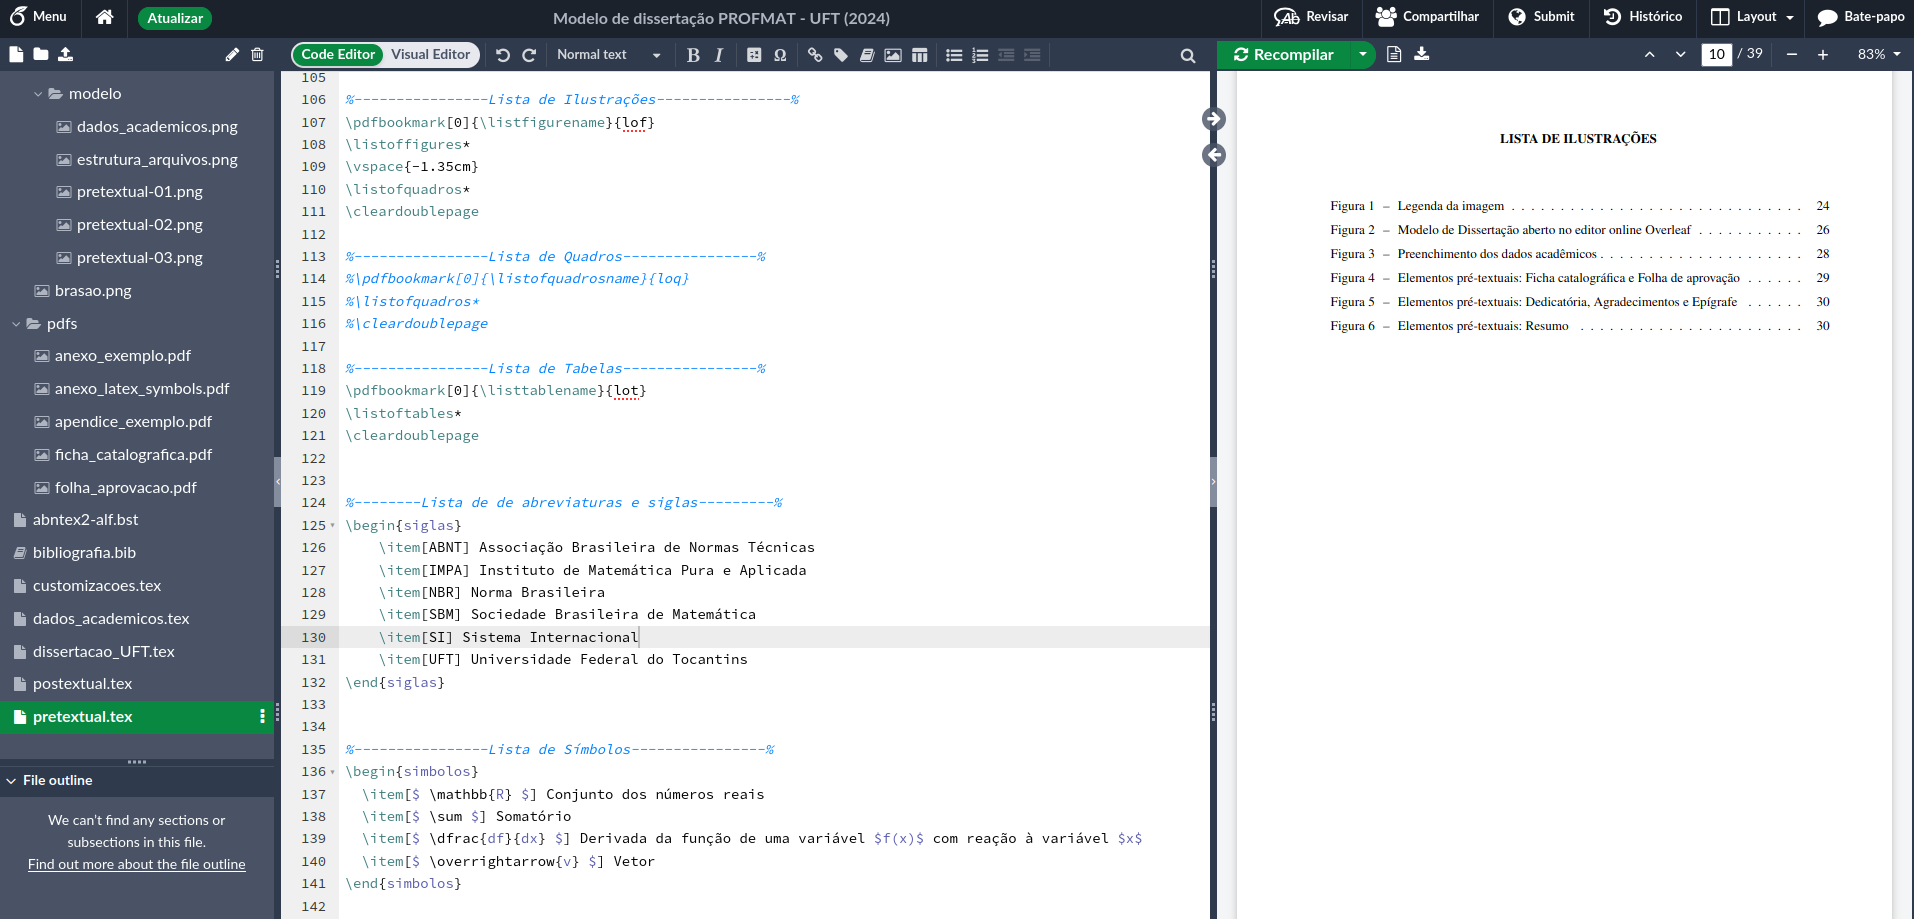
\includegraphics[width=0.9\textwidth]{img/modelo/pretextual-04.png}
    \\
    \caption*{\small{Fonte: Autor (20XX)}}
    \label{fig:pretextual-04}
\end{figure}

Observe que a Listas de Ilustrações, a Lista de Quadros e a Lista de Tabelas são criadas automaticamente, à medida que estes elementos são incluídos no texto do trabalho. Portanto, apenas a Lista de Abreviaturas e Siglas  e a Lista de Símbolos requerem preenchimento manual pelo autor do trabalho. Alguns exemplos podem ser encontrados no arquivo \verb|pretextual.tex|.

Para finalizar a parte de elementos pré-textuais, tem-se o sumário. À  medida que o autor adiciona novos capítulos (\verb|\chapter{|), seções (\verb|\section|) e subseções (\verb|\subsection|), o sumário será atualizado automaticamente.

\section*{Elementos Textuais}

Conforme norma ABNT NBR 14724:2011, os elementos textuais são compostos por ``uma parte introdutória, na qual são informados os objetivos do trabalho e as razões de sua elaboração; o desenvolvimento, que apresenta a pesquisa ou estudo realizado; e uma parte conclusiva'' \cite[p.~8]{nbr14724}.

Para uma melhor organização do trabalho, a parte textual da dissertação foi dividida em capítulos: \verb|cap_01.tex|, \verb|cap_02.tex|, \verb|cap_03.tex|, \verb|cap_04.tex| e \verb|cap_05.tex| dentro na pasta \verb|capitulos|.  Note que o carregamento desses arquivos para a dissertação é feito por meio do comando \verb|\include| no arquivo principal \verb|dissertacao_UFT.tex|, como mostrado na Figura \ref{fig:textual-01}.

\begin{figure}[H]
    \centering
    \caption{Elementos textuais}
    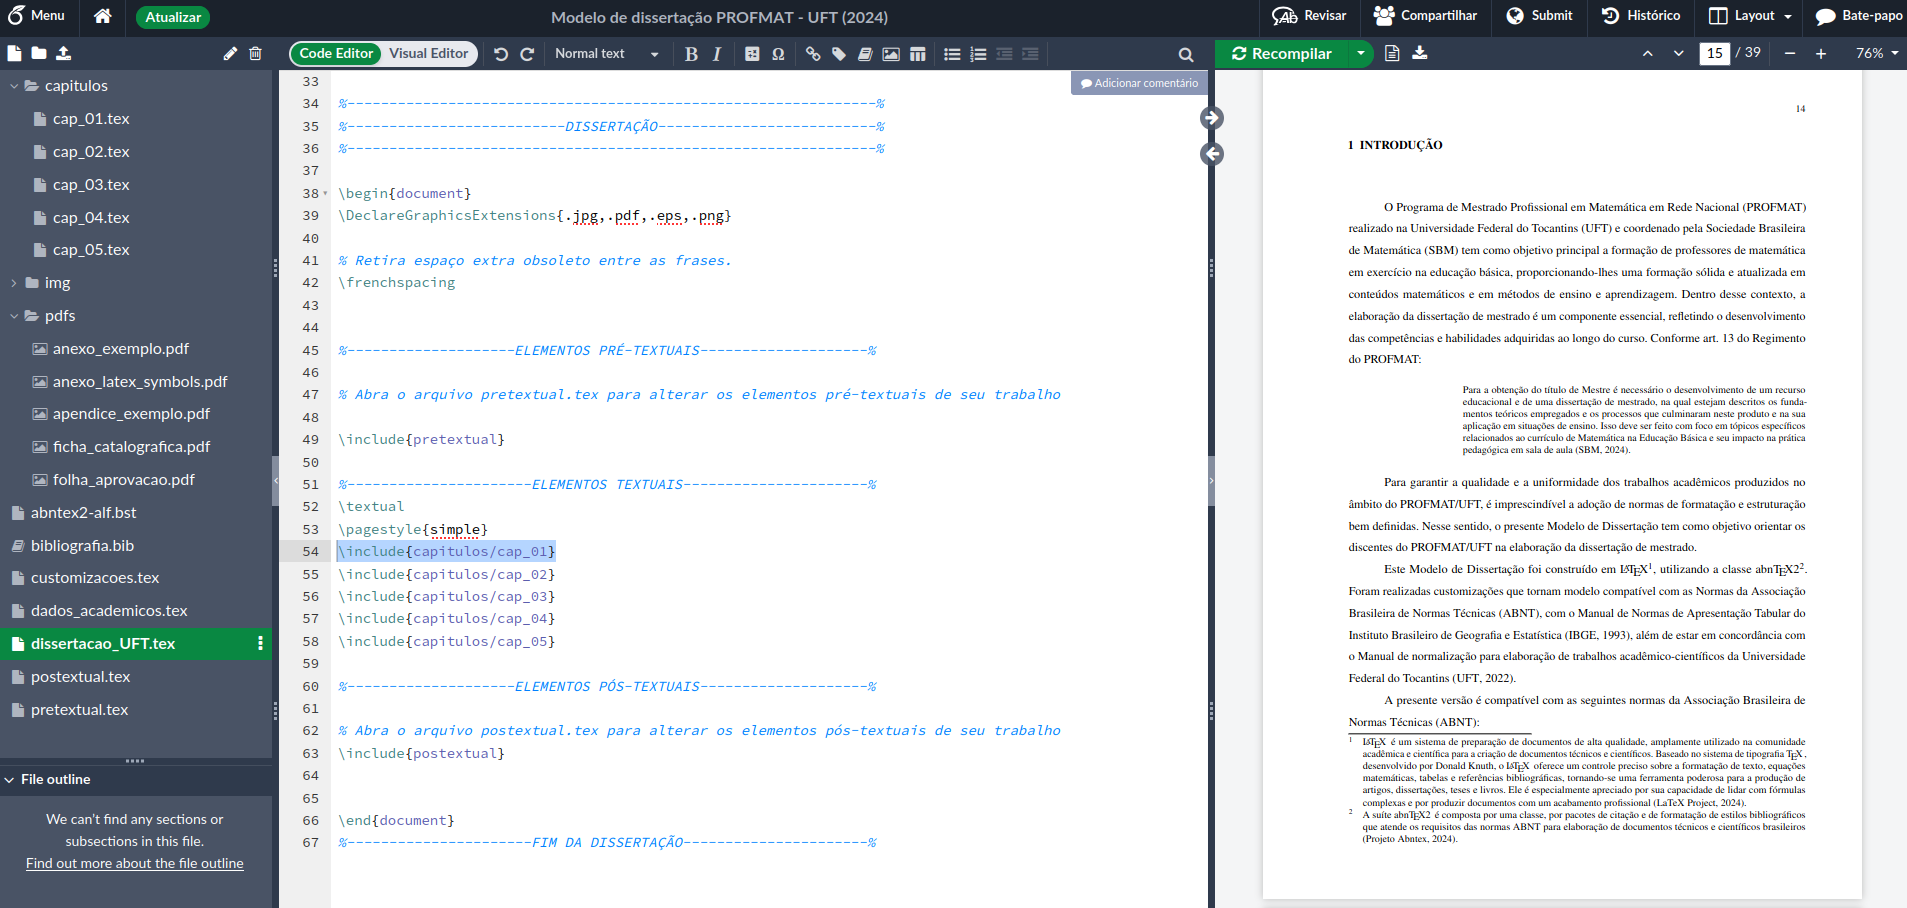
\includegraphics[width=0.9\textwidth]{img/modelo/textual-01.png}
    \\
    \caption*{\small{Fonte: Autor (20XX)}}
    \label{fig:textual-01}
\end{figure}

Observe na Figura \ref{fig:textual-01} que para a inclusão do arquivo \verb|cap_01.tex| foi utilizado o comando \verb|%----------------Cap_01----------------%

\chapter{INTRODUÇÃO}

O Programa de Mestrado Profissional em Matemática em Rede Nacional (PROFMAT) realizado na Universidade Federal do Tocantins (UFT) e  coordenado pela Sociedade Brasileira de Matemática (SBM) tem como objetivo principal a formação de professores de matemática em exercício na educação básica, proporcionando-lhes uma formação sólida e atualizada em conteúdos matemáticos e em métodos de ensino e aprendizagem. Dentro desse contexto, a elaboração da dissertação de mestrado é um componente essencial, refletindo o desenvolvimento das competências e habilidades adquiridas ao longo do curso. Conforme art. 13 do Regimento do PROFMAT:

\begin{citacao}
    Para a obtenção do título de Mestre é necessário o desenvolvimento de um recurso educacional e de uma dissertação de mestrado, na qual estejam descritos os fundamentos teóricos empregados e os processos que culminaram neste produto e na sua aplicação em situações de ensino. Isso deve ser feito com foco em tópicos específicos relacionados ao currículo de Matemática na Educação Básica e seu impacto na prática pedagógica em sala de aula \cite{profmat_regimento}.
\end{citacao}
 

Para garantir a qualidade e a uniformidade dos trabalhos acadêmicos produzidos no âmbito do PROFMAT/UFT, é imprescindível a adoção de normas de formatação e estruturação bem definidas. Nesse sentido, o presente Modelo de Dissertação tem como objetivo orientar os discentes do PROFMAT/UFT na elaboração da dissertação de mestrado.

Este Modelo de Dissertação foi construído em \LaTeX \footnote{\LaTeX\, é um sistema de preparação de documentos de alta qualidade, amplamente utilizado na comunidade acadêmica e científica para a criação de documentos técnicos e científicos. Baseado no sistema de tipografia \TeX\,, desenvolvido por Donald Knuth, o \LaTeX\, oferece um controle preciso sobre a formatação de texto, equações matemáticas, tabelas e referências bibliográficas, tornando-se uma ferramenta poderosa para a produção de artigos, dissertações, teses e livros. Ele é especialmente apreciado por sua capacidade de lidar com fórmulas complexas e por produzir documentos com um acabamento profissional \cite{latex-projeto}.}, utilizando a classe \abnTeX\footnote{A suíte \abnTeX\, é composta por uma classe, por pacotes de citação e de formatação de estilos bibliográficos que atende os requisitos das normas ABNT para elaboração de documentos técnicos e científicos brasileiros \cite{abntex-projeto}.}. Foram realizadas customizações que tornam modelo compatível com as Normas da Associação Brasileira de Normas Técnicas (ABNT), com o Manual de Normas de Apresentação Tabular do Instituto Brasileiro de Geografia e Estatística \cite{ManualIBGE}, além de estar em concordância com o Manual de normalização para elaboração de trabalhos acadêmico-científicos da Universidade Federal do Tocantins \cite{ManualUFT}.

Este Modelo de Dissertação é compatível com as seguintes normas da Associação Brasileira de Normas Técnicas (ABNT):

\begin{itemize}
	\item ABNT NBR 14724:2011 - Informação
e documentação: trabalhos acadêmicos: apresentação \cite{nbr14724};

    \item ABNT NBR 10520:2023 - Informação
e documentação: citações em documentos: apresentação \cite{nbr10520};

	\item ABNT NBR 6023:2018 - Informação
e documentação: referências: elaboração \cite{nbr6023};

    \item ABNT NBR 6024:2012 - Informação
e documentação: Numeração progressiva das seções de um documento: apresentação \cite{nbr6024};
 
	

	\item ABNT NBR 6027:2012 - Informação
e documentação: sumário: apresentação \cite{nbr6027}.

    \item ABNT NBR 6028:2021 - Informação
e documentação: resumo, resenha e recensão: apresentação \cite{nbr6028};

    	\item ABNT NBR 6034:2011 - Informação
e documentação: índice: apresentação \cite{nbr6034}.
\end{itemize} 

Assim, espera-se que os discentes do PROFMAT/UFT possam produzir documentos acadêmicos que atendam aos padrões exigidos pela comunidade científica, contribuindo para a sua formação e para o avanço do conhecimento na área de ensino da matemática.

No que segue, o modelo de dissertação será descrito em detalhes.


|, em que dentro das chaves foi passado o caminho até o referido arquivo, sem a extensão \textit{.tex}. Dois fatos importantes sobre a inclusão de arquivos são:
\begin{itemize}
    \item A ordem em que os arquivos aparecerão na dissertação \textbf{não} depende do nome com que foram salvos e sim da ordem em que foram incluídos no arquivo principal. 
    \item Para adicionar um novo arquivo, por exemplo, um arquivo de nome \verb|cap_06.tex|, crie esse arquivo dentro da pasta reservada \verb|capitulos|. Depois disso, inclua o comando \verb|\include{capitulos/cap_06}| no arquivo principal \verb|dissertacao_UFT.tex|, 
\end{itemize}


\section*{Elementos Pós-textuais}

Os elementos pós-textuais correspondem às referências, apêndices e anexos do trabalho acadêmico. Destes, apenas as referências são um elemento obrigatório segundo a norma ABNT NBR 14724:2011 \cite{nbr14724}.  Para editar os elementos pós-textuais, abra o arquivo \verb|postextual.tex|.




\chapter{Exemplo de apêndice em pdf}\label{apend:exemplo}
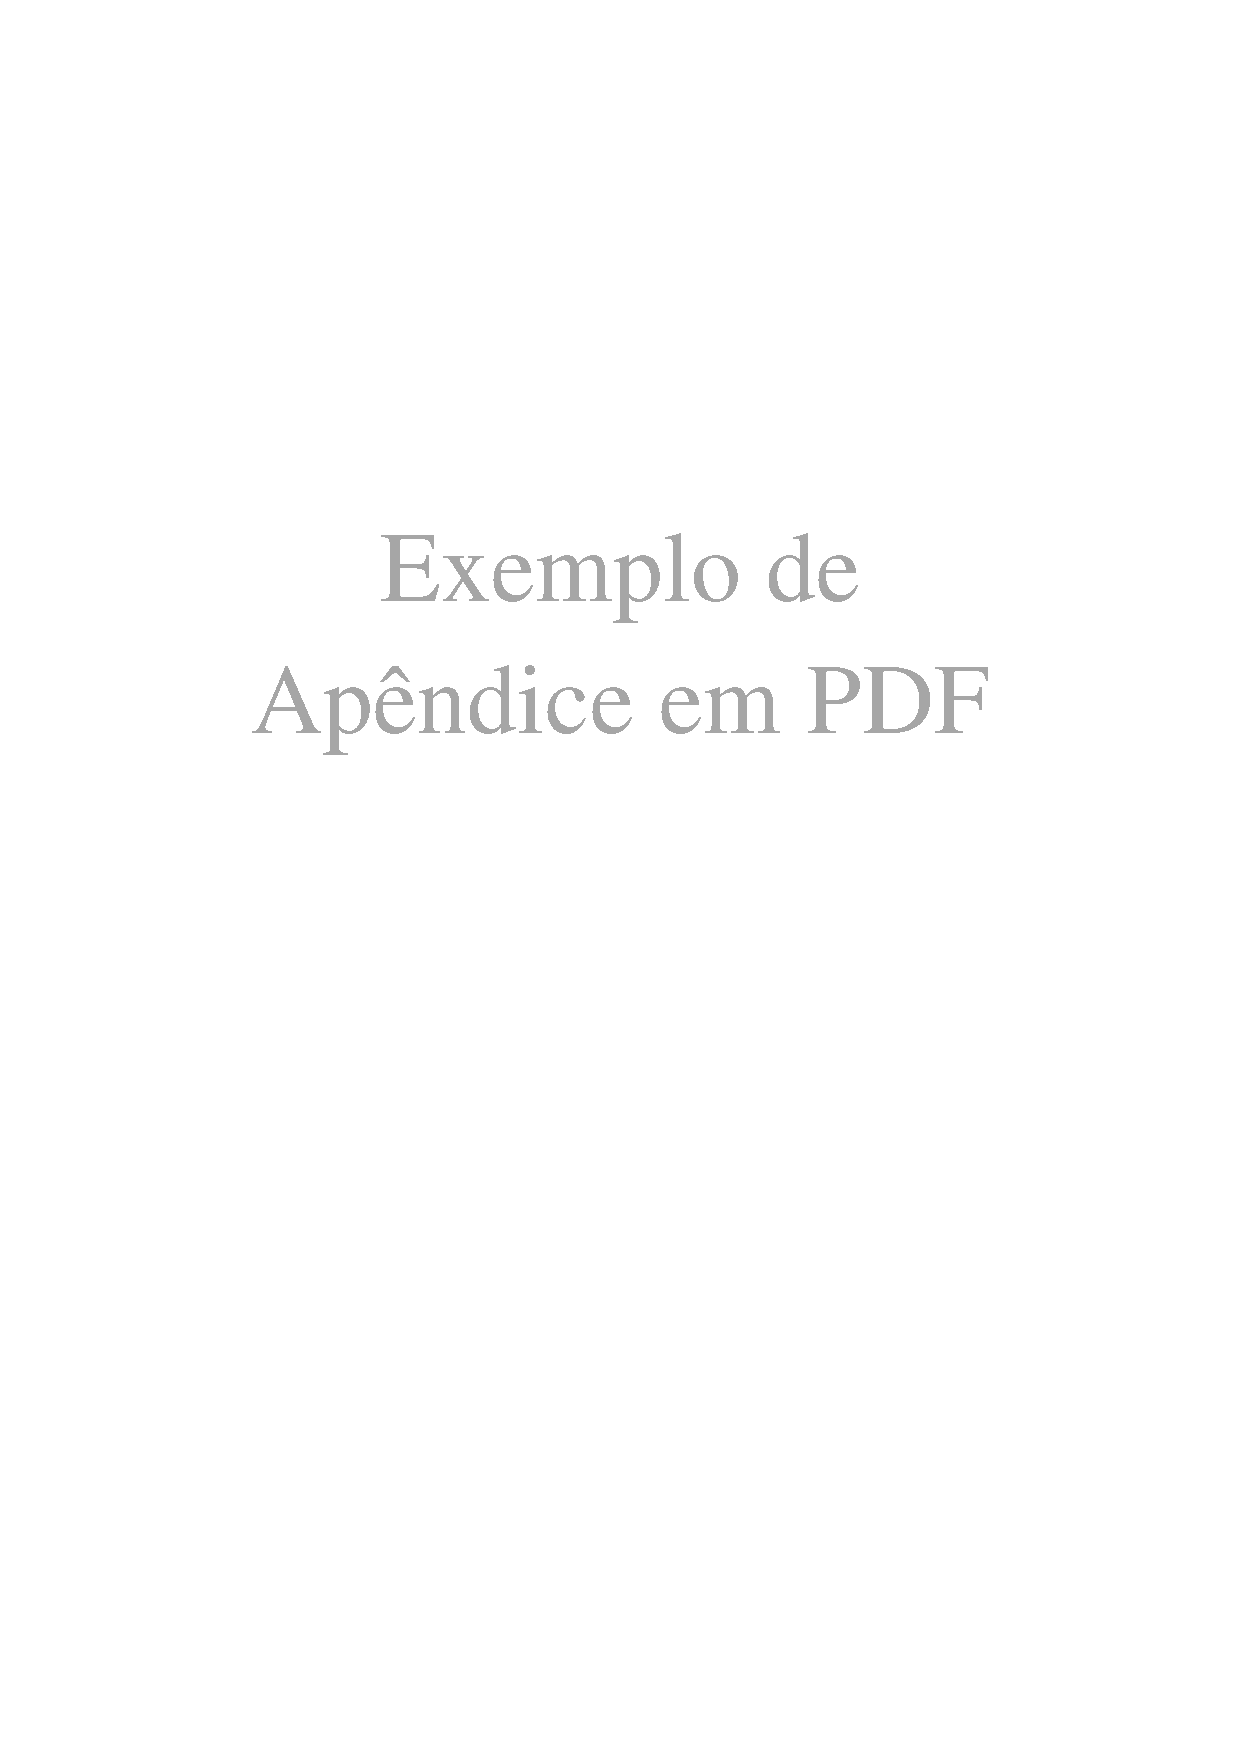
\includepdf[pages=-]{pdfs/apendice_exemplo.pdf}
\end{apendicesenv}

\begin{anexosenv}


%-----------------------------Anexos-----------------------------%
% Imprime uma página indicando o início dos anexos

% ---
\chapter{Símbolos matemáticos em LaTeX}\label{anexo:symbols}
% ---
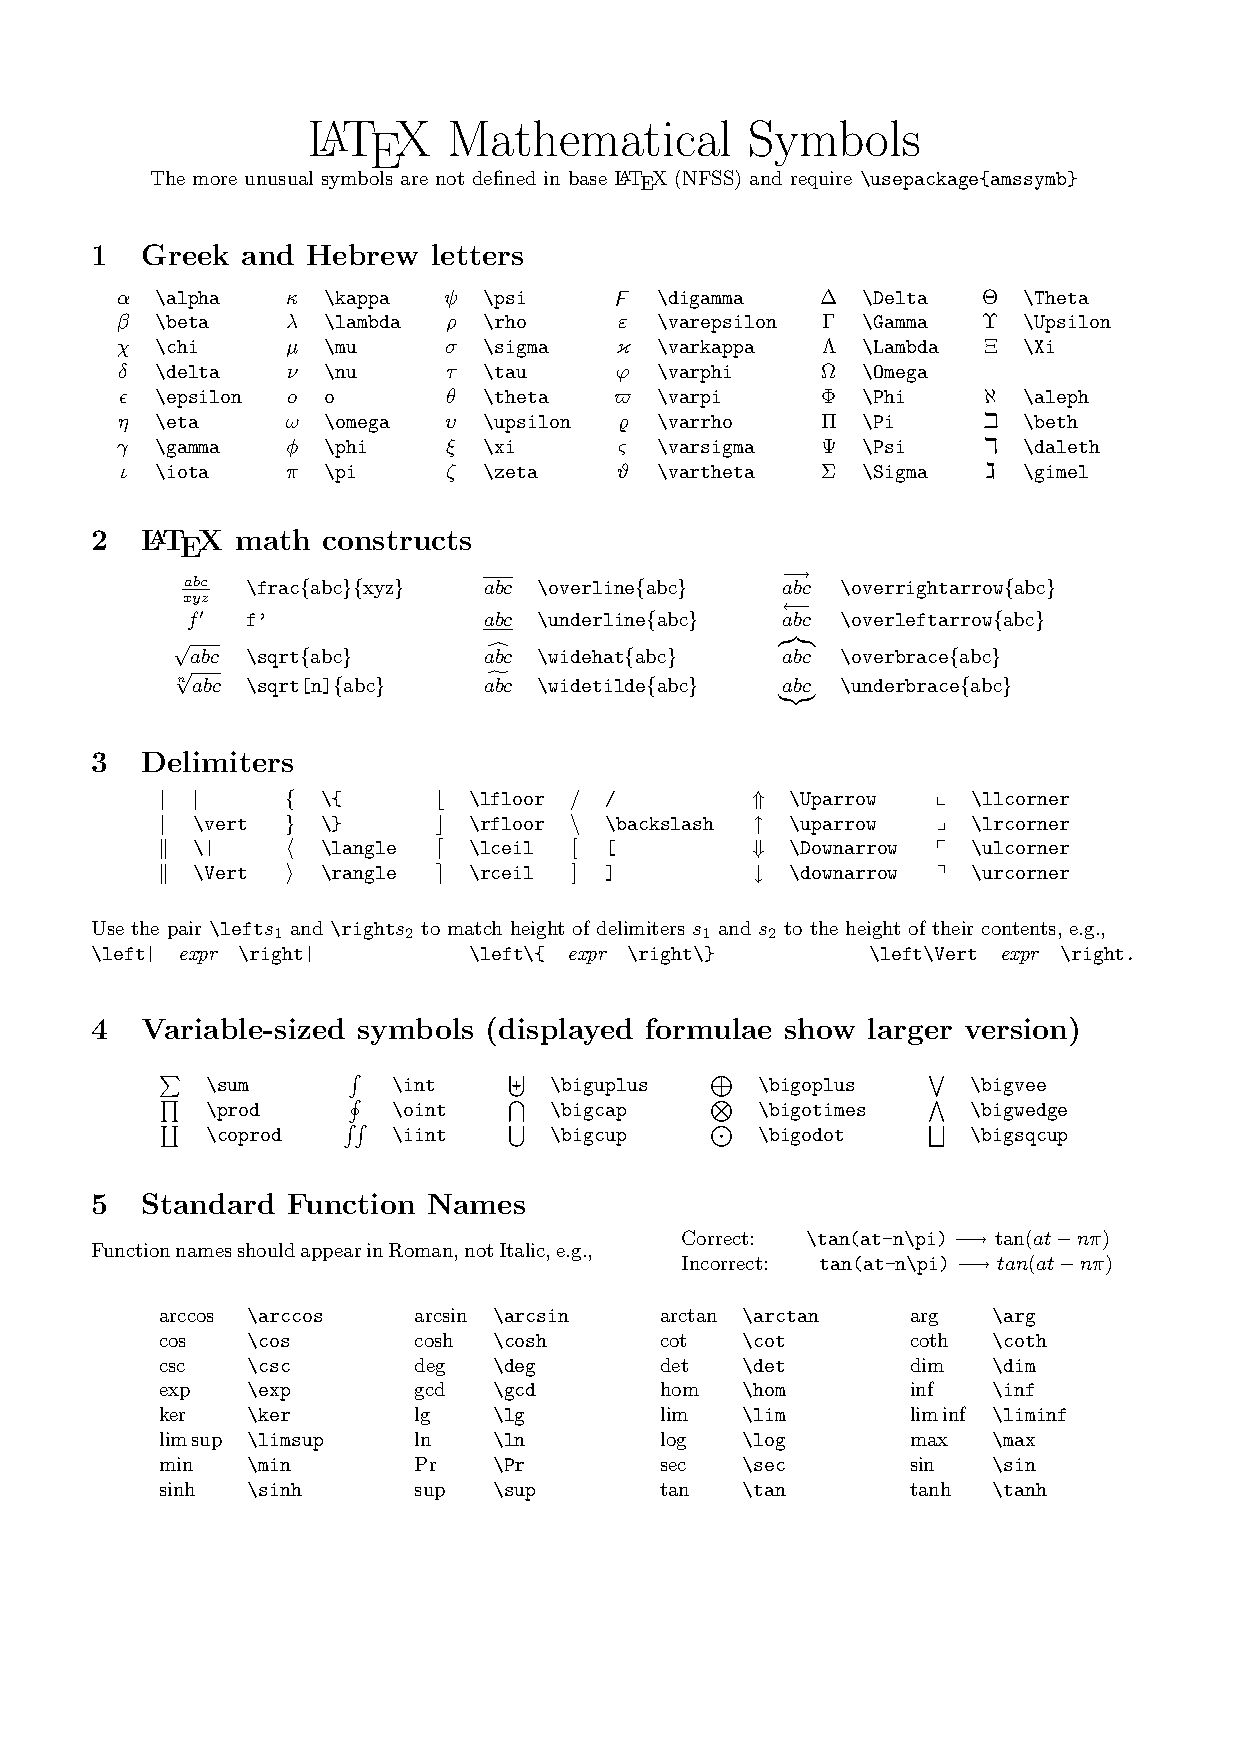
\includepdf[pages=-]{pdfs/anexo_latex_symbols.pdf}
\end{anexosenv}
